\documentclass[a4paper,11pt]{report}

\usepackage{fancyhdr}
\usepackage{graphicx}
\usepackage[top=1.5cm, bottom=3cm, left=2.5cm, right=2.5cm]{geometry} % Adjust margins
\usepackage{setspace}
\usepackage[linktoc=page]{hyperref}
\usepackage{sectsty}
\chapterfont{\centering}
\usepackage{makeidx}
\usepackage{url}
\usepackage[square,sort,comma,numbers]{natbib}
\usepackage{framed}
\usepackage{longtable}
\usepackage{amsfonts}
\usepackage{amsmath}
\usepackage{booktabs} % For better looking tables
\usepackage{array} 
\usepackage[noend,ruled,noline,linesnumbered,algochapter]{algorithm2e}

% Set header and footer space
\setlength{\headheight}{0pt} % Remove extra height in header
\setlength{\headsep}{0.5cm} % Reduce space between header and text

% Title Page
\begin{document}

% Fancy header and footer settings
\pagestyle{fancy}
\fancypagestyle{plain}{%
    \fancyhf{} % clear all header and footer fields
    \renewcommand{\headrulewidth}{0pt}
    \fancyfoot[L]{\textit{©Daffodil International University}}
    \fancyfoot[R]{\thepage}
}

\fancyhf{} % clear all header and footer fields
\renewcommand{\headrulewidth}{0pt}
\fancyfoot[L]{\textit{©Daffodil International University}}
\fancyfoot[R]{\thepage}

% Set headers: chapter on the left, section on the right
\fancyhead[L]{\nouppercase{\leftmark}} % Chapter title on the left
\fancyhead[R]{\nouppercase{\rightmark}} % Section title on the right

% Title Page
\begin{titlepage}

\vspace*{2cm} % Adjust this value to increase the header space

\begin{center}
{\huge\bf 12 Volt Battery Level Indicator }
\end{center}

\vspace{2cm}

\begin{center}
\Large \bf Submitted By
\end{center}

\vspace{.1cm}

\begin{table}[h!]
\centering
\begin{tabular}{|c|c|}
\hline
\textbf{      Student Name      } & \textbf{  Student ID  } \\
\hline
 Jannatul Ferdaues & 232-15-689  \\
\hline
 Student-1 Name & Student-1 ID \\
\hline
Student-3 Name & Student-3 ID \\
\hline
Student-4 Name & Student-4 ID \\
\hline
Student-5 Name & Student-5 ID \\
\hline
\end{tabular}
\end{table}

\vspace{2cm}

\begin{center}
{\Large\bf LAB PROJECT REPORT}\\
\vspace{0.2cm}
\Large This Report Presented in Partial Fulfillment of the course  \textbf{CSE215:  Electrical Device and circuit in the Computer Science and Engineering Department}
\end{center}

\vspace{2cm}

\begin{center}

\includegraphics[scale=0.5]{./figures/DIU Logo}
\end{center}

\begin{center}
	\Large\textbf{DAFFODIL INTERNATIONAL UNIVERSITY}\\
 \textbf{\textsc{Dhaka, Bangladesh}}
\end{center}

\begin{center}
\textbf{\today}
\end{center}

\end{titlepage}

\clearpage

% Set Roman page numbering for initial pages
\pagenumbering{roman}
\setcounter{page}{1}

% Declaration-------------------------
\phantomsection

\vspace*{1.5cm} 

\addcontentsline{toc}{chapter}{Declaration}

\begin{center}
    {\LARGE \textbf{DECLARATION}}\\
   % \line(1,0){430}
\end{center}

\onehalfspacing

\noindent We hereby declare that this lab project has been done by us under the supervision of \textbf{Name of the course teacher}, \textbf{course teacher's Designation}, Department of Computer Science and Engineering, Daffodil International University. We also declare that neither this project nor any part of this project has been submitted elsewhere as lab projects. 

\vspace{.8cm}

\noindent \textbf{Submitted To:} \\[1cm]
\usepackage{graphicx}
\begin{figure}[h!]
  \caption{A picture of a gull.}
  \centering
  \includegraphics[width=0.5\textwidth]{sir.png}
\end{figure}
\noindent\rule{6cm}{0.4pt}\\
\textbf{Course Teacher's Name} \\
Designation \\
Department of Computer Science and Engineering \\
Daffodil International University \\

\vspace{.5cm}

% Table
\begin{center}
    \textbf{Submitted by}
\end{center}

\vspace{.2cm}

\begin{table}[h!]
\centering
\renewcommand{\arraystretch}{3} % Increase row height for more space
\setlength{\tabcolsep}{10pt} % Adjust column spacing

\begin{tabular}{|p{0.48\textwidth}|p{0.35\textwidth}|} % Equal column widths

\hline
\multicolumn{2}{|c|}{
    \begin{minipage}{\linewidth}
        \centering
        \vspace{1.5cm} % Space above the name for signature
        \rule{6cm}{0.4pt} % Signature line
        \\
        \textbf{Student Name} \\ Student ID: \\ Dept. of CSE, DIU
    \end{minipage}
} \\
\hline

\begin{minipage}{\linewidth}
    \centering
    \vspace{1.5cm} % Space above the name for signature
    \rule{6cm}{0.4pt} % Signature line
    \\
    \textbf{Student Name} \\ Student ID: \\ Dept. of CSE, DIU
\end{minipage} &

\begin{minipage}{\linewidth}
    \centering
    \vspace{1.5cm} % Space above the name for signature
    \rule{6cm}{0.4pt} % Signature line
    \\
    \textbf{Student Name} \\ Student ID: \\ Dept. of CSE, DIU
\end{minipage} \\
\hline

\begin{minipage}{\linewidth}
    \centering
    \vspace{1.5cm} % Space above the name for signature
    \rule{6cm}{0.4pt} % Signature line
    \\
    \textbf{S} \\ Student ID: \\ Dept. of CSE, DIU
\end{minipage} &

\begin{minipage}{\linewidth}
    \centering
    \vspace{1.5cm} % Space above the name for signature
    \rule{6cm}{0.4pt} % Signature line
    \\
    \textbf{Student Name} \\ Student ID: \\ Dept. of CSE, DIU
\end{minipage} \\
\hline

\end{tabular}

\end{table}


\newpage
%Abstract
\phantomsection
\vspace*{1.5cm} 
\addcontentsline{toc}{chapter}{Course \& Program Outcome}
\setlength{\headheight}{14pt}
\begin{center}
	{\LARGE \bf COURSE \& PROGRAM OUTCOME}\\
	%\line(1,0){430}
\vspace*{1.5cm} 
\begin{flushleft}
The following course have course outcomes as following:.
\end{flushleft}

% table of CO's....................
\begin{table}[h!]
\centering
\caption{Course Outcome Statements}
\vspace{0.1cm} % Adds a 0.5 cm space between the caption and the table
\begin{tabular}{|p{0.06\textwidth}|p{.9\textwidth}|}
\hline
\textbf{CO's} & \textbf{Statements} \\
\hline
CO1 & \textbf{Define} and \textbf{Relate} classes, objects, members of the class, and relationships among them needed for solving specific problems \\
\hline
CO2 & \textbf{Formulate} knowledge of object-oriented programming and Java in problem solving \\
\hline
CO3 & \textbf{Analyze} Unified Modeling Language (UML) models to \textbf{Present} a specific problem \\
\hline
CO4 & \textbf{Develop} solutions for real-world complex problems \textbf{applying} OOP concepts while evaluating their effectiveness based on industry standards. \\
\hline
\end{tabular}
\end{table}

\vspace{1cm}
%----------------------------
% table for Mapping of CO, PO, Blooms, KP and CEP---------
\begin{table}[h!]
\centering
\caption{Mapping of CO, PO, Blooms, KP and CEP}
\begin{tabular}{|>{\centering\arraybackslash}m{2cm}|>{\centering\arraybackslash}m{2cm}|>{\centering\arraybackslash}m{2cm}|>{\centering\arraybackslash}m{2cm}|>{\centering\arraybackslash}m{2cm}|}
\hline
\textbf{CO} & \textbf{PO} & \textbf{Blooms} & \textbf{KP} & \textbf{CEP} \\
\hline
CO1 & PO1 & C1, C2 & KP3 & EP1,EP3 \\
\hline
CO2 & PO2 & C2 & KP3 & EP1,EP3 \\
\hline
CO3 & PO3 & C4, A1 & KP3 &EP1,EP2 \\
\hline
CO4 & PO3 & C3, C6, A3, P3 & KP4 & EP1,EP3 \\
\hline
\end{tabular}
\end{table}
\begin{flushleft}
The mapping justification of this table is provided in section \textbf{4.3.1}, \textbf{4.3.2} and \textbf{4.3.3}.
\end{flushleft}



\setlength
{\headheight}{12pt}


% Table of contents
\renewcommand*\contentsname{Table of Contents}
\tableofcontents
\clearpage

\renewcommand\bibname{References}
\clearpage

% Start of report and chapters
\pagenumbering{arabic} % Switch to Arabic numbering
\setcounter{page}{1}

% Reapply header and footer settings for the main content
\fancyhf{} % clear header and footer
\fancyfoot[L]{\textit{©Daffodil International University}}
\fancyfoot[R]{\thepage}
\fancyhead[L]{\nouppercase{\leftmark}} % Chapter title on the left
\fancyhead[R]{\nouppercase{\rightmark}} % Section title on the right

% Chapters content...................................
\chapter{Introduction}

%This is for reference only. Delete before finalization

\noindent This chapter provides a brief description of the project’s objectives, motivation and results. 
\end{center}
%This is for reference only. Delete before finalization


% Start sections and sub-sections

\section{Introduction}
In today's world, batteries are an essential thing to operate various devices and systems. 12V batteries are widely used in various vehicles ranging from backup power supply and renewable energy systems—however, excessive charging or deep discharging of the battery results in reduced battery life. 
12V battery level indicator, the main objective of the project is to monitor the charge level of a battery and ensure effective use, maintenance, and power supply of the battery. The LED lights used in the project provide an idea of the current power supply and charge of the battery. This project generally contributes significantly to daily battery level monitoring and economical usage \cite{b4}.

\section{Motivation}
Currently, the need for batteries is immense for the use of modern devices and for uninterrupted power supply in various fields. Battery mismanagement (e.g., deep discharging and overcharging) for various reasons can shorten battery life and reduce performance. As a result, users face financial loss for battery replacement. This disrupts uninterrupted power flow and increases the risk of power outages. The project aims to encourage the use of renewable energy and create simple, budget-friendly solutions. This will result in financial savings and less generation of electronic waste \cite{b5}.

\section{Objectives}
Generally the purpose of this project is,\newline
 1. Designing a cost-effective, easy-to-use, reliable 12V battery level indicator.\newline
 2. Making the battery charge level visible and understandable through the use of LED lights in the circuit.\newline
 3. Ensuring compatibility with various applications including vehicles, backup systems and solar panels.\newline
 4. Making users aware of energy conservation, saving and battery maintenance.\newline 
These objectives aim to solve everyday problems technologically and make it easier to use \cite{b6}.

\section{Feasibility Study}
Feasibility study is done to test the feasibility of the project before starting the design. It can be seen that the necessary parts of the project like resistors, LEDs, diodes, transistors are cheap and readily available. The "Proteus" tool is used for circuit accuracy testing and these basic kits used for prototyping simplify the process. The project is considered cost-effective due to low cost of prototyping. And being affordable makes it suitable for many users. And because of the simplicity of the design, it can be easily modified to work with different types of batteries in the future \cite{b7}.

\section{Gap Analysis}
\textbf{Existing Work :}\newline
1. Many battery level indicators exist, but they are often expensive or lack features such as clear visualization or customizable alerts.\newline
2. Some existing models are not user-friendly and may require advanced technical knowledge to operate.\newline
3. Most affordable indicators fail to provide precise readings or sustained performance.\newline
\textbf{Our Approach :}\newline
1. The goal of this project is to develop a low-cost, user-friendly, and accurate 12V battery level indicator.\newline
2. The focus will be on developing a device that uses common components such as LEDs or LCDs to make the battery status clearly visible to any user.\newline
3. The disadvantage of this project is that if the current flows more than 25V, there is a possibility of burning the circuit \cite{b8}.
\section{Project Outcome}
1. A working prototype of a 12-volt battery level indicator.\newline
2. A cost-efficient design suitable for mass production.\newline
3. Improved battery management for automotive, solar, and industrial applications.\newline
4. Improved user convenience through real-time charge monitoring.\newline
5. Increased battery life by preventing overcharging or deep discharging.\newline
6. A design that is easy to replicate and modify for different applications \cite{b9}.


\chapter{Proposed Methodology/Architecture}
\phantomsection

%This is for reference only. Delete before finalization


\begin{center}
    

For every project, the methodology and architecture are very important. In this chapter, the requirements, design, feasibility, and overall plan will be discussed. 
    
\end{center}
%This is for reference only. Delete before finalization



\section{Requirement Analysis \& Design Specification}
\subsection{Requirement Analysis}
 The BC547 transistor and Zener diode are mainly used to create the circuit. The BC547 transistor is particularly used because it works in high-fidelity amplification and minimal signal interference. In this circuit, three different kinds of Zener diodes: 7.5 volts, 10 volts, and 12 volts are used. Six resistors, of two different types, are needed to complete the circuit: 1k ohms and 10k ohms. Working process based on week: \newline
 \textbf{Week 1:}\newline
     \textbf{1. Requirement analysis and circuit design:}\newline
     This involves a close analysis of the project requirements to identify the circuit's scope and functionality. It involves listing the basic circuit design according to the project requirements.\newline
    \textbf{2. Component procurement:}\newline
    After the design of the circuit is finalized, identify all the required components. The components should be high-quality parts sourced in conformation to specifications in the design to ensure no hassle in implementing the circuit.\newline
 \textbf{Week 2:}\newline
    \textbf{1. Circuit simulation and testing on a breadboard:}\newline
    In this stage, the software tools are used to simulate the circuit design to validate it. After successful simulation, the design is assembled on a breadboard, where it is tested for practical performance and any initial issues are identified and resolved.\newline
 \textbf{Week 3:}\newline
    \textbf{1. Prototype refinement and final testing:}\newline
    After receiving the result from the testing with a breadboard, the prototype is refined for further design flaws or inefficiencies. A final version of the prototype will be rigorously tested to confirm that it indeed fits the specifications and works well.\newline
    \newline
    \newline
 \textbf{Week 4:}\newline
    \textbf{1. Documentation and report preparation:}\newline
    In the final stage, everything in the project is documented in detail, be it design processes, testing, or results. A report detailing the project and findings will be prepared for presentation or submission.\newline
\subsection{Design Specification}
\onehalfspacing

 Firstly, a breadboard is needed as a base for the circuit. After that, take the BC547 resistors and place them on the board. Then one side of the 10k ohm resistor is connected to the base pin of the transistor and the other side with the Zener diode. The Zener diode must be placed in reverse order. For the collector pin put the positive side of the LED with the collector pin and the negative side with the 1k ohm resistor. Then connect the emitter pin with the negative side and connect the second side of the 1k ohm resistor with the positive supply source. The black color wire is for identifying the negative connection and the red color wire is for identifying the positive connection of the circuit \cite{b3}. 
\section{Feasibility Study}

\subsection{Overview}
 In this project, Zener diodes are used as a main component, because they give the best outcome in reverse bias. The diode begins to conduct current or voltage when it exceeds the voltage of the knee. Thus, the Zener diode diverts the current that passes through it and works as a stabilizer \cite{b2}. This demonstrates the Zener diode's voltage management capability. The project gives the desired outcome by connecting three Zener diodes in a series connection in a reverse bias. And also connecting the two 9-voltage batteries in a series connection to make an 18-volt battery   \cite{Electronics_Projects_for_Dummies}.
\vspace{.1cm}

\begin{table}[h!]
\centering
\begin{tabular}{|  c  |c|}
\hline
\textbf{      Item      } & \textbf{  Type  }  \\
\hline
Transistor &   BC547   \\
\hline
 Zener Diode  & 7v, 10v, 12v     \\

\hline
 Resistor & 1k ohm  \\
\hline
 Resistor & 10k ohm  \\
\hline
Breadboard  & Big size  \\
\hline
LED Light  & Red, Yellow, Green  \\
\hline
Male to Male Jumper wire  & Black, Red\\

\hline
\end{tabular}
\caption{Using Items }
\end{table}



\subsection{Proposed Methodology}
The purpose of this project is to design and build a voltage level indicator for a 12V battery. The primary purpose is to monitor the charge level of a 12v battery, allowing users to determine the remaining battery life and take appropriate actions such as recharging. If the battery level is higher than or equal to 33\%, the LED light connected to a 7v Zener diode will glow. If the battery level is higher than or equal to 66\%, the LED light connected to a 10v Zener diode will glow. If the battery level is equal to 100\%, the LED light connected to a 12v Zener diode will glow. transistor BC517 which is two transistors integrated into one single component; it was used identically as BC547 in with cascade consisting of two BC547 transistors (right) \cite{2}.


\subsection{Costing }

The table of cost analysis is given in table 2.3.
\begin{table}[h!]
\centering
\begin{tabular}{|  c  |c|c|}
\hline
\textbf{      Item      } & \textbf{  Required piece  } & \textbf{  Price  }  \\
\hline
 BC547 Transistor &  3 pieces & 15 taka    \\
\hline
 Zener Diode  &3 pieces  & 15 Taka    \\

\hline
1k ohm Resistor & 3 pieces & 6 Taka    \\
\hline
10k ohm Resistor & 3 pieces & 21 Taka \\
\hline
Breadboard  & 1 piece & 180 Taka  \\
\hline
LED Light  & 3 pieces & 10 Taka  \\
\hline
9-volt battery & 2 pieces & 150 tk\\
\hline
Male to Male Jumper wire  & 10 pieces & 15 Taka\\
\hline
 & & \textbf{Total cost: 312 Taka}\\
\hline
\end{tabular}
\caption{Cost Analysis }
\end{table}

The alternative Costing table is shown in table 2.3.
\begin{table}[h!]
\centering
\begin{tabular}{|  c  |c|c|c|}
\hline
\textbf{      Item      } & \textbf{  Quantity  } & \textbf{ Unit Price (BDT) } & \textbf{  Total Price (BDT)  }  \\
\hline
 BC547 Transistor &  3  & 5 & 15    \\
\hline
 Resistors &  6 &	1 &	6   \\

\hline
LEDs &	3 &	5 &	15    \\
\hline
Zener Diode	 & 3  &	10 &	30 \\
\hline
Breadboard  & 1 & 180 &180 \\
\hline
Male to Male Jumper wire  & 1 set & 10  & 15 \\
\hline
Battery Clips/Connectors	& 1 &	15 &	15\\
\hline
12-volt battery & 1 & 1000 & 1000\\
\hline
 & &  &\textbf{Total cost: 1275 Taka}\\
\hline

\end{tabular}
\caption{Cost Analysis }
\end{table}
\newline
\newline
\newline
\newline
\newline
\pagebreak
\subsection{System Design}

The circuit design is shown in Figure: 2.1.
\begin{figure}[h!] % 'h' for placing it "here"
    \centering
    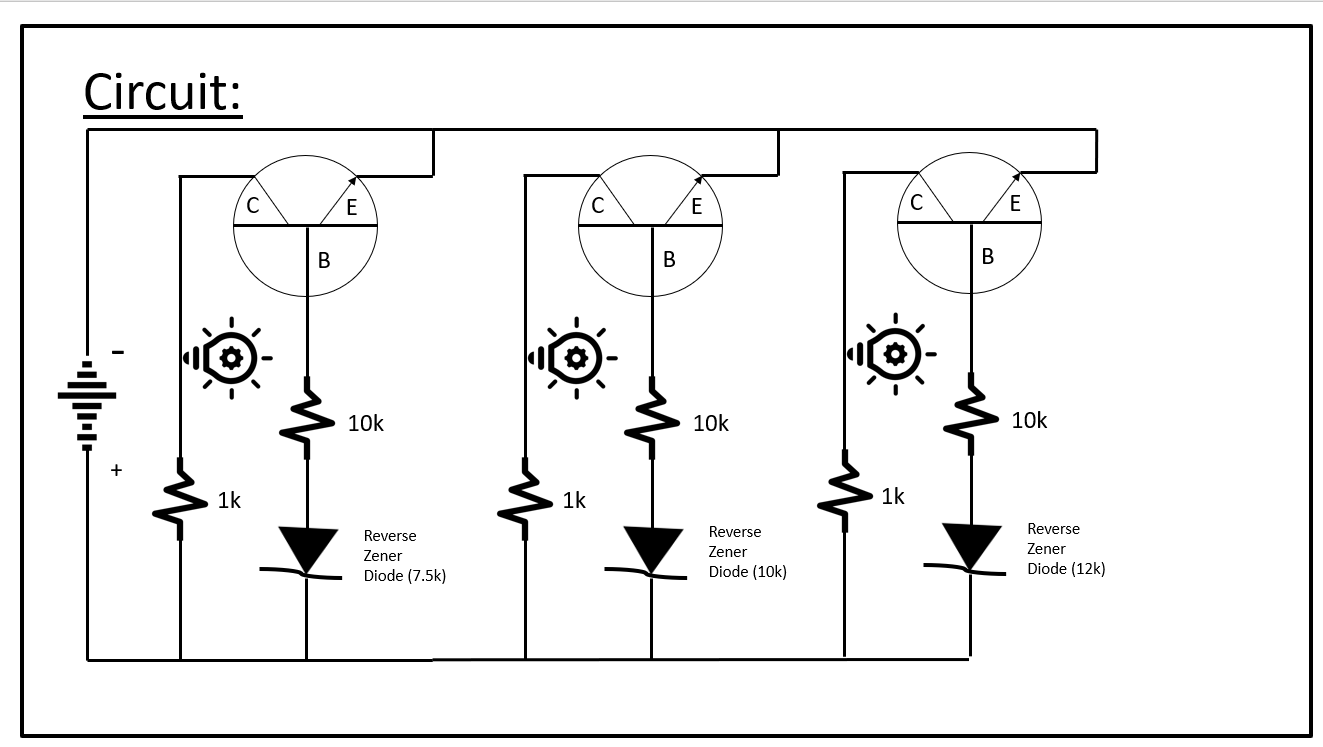
\includegraphics[width=0.5\textwidth]{Diagram.png} % Replace 'diagram.png' with your image file
    \caption{12v Battery Level Indicator}
    \label{fig:sample}
\end{figure}
\subsection{Workflow}
The workflow is shown in Figure: 2.2\newline
\begin{figure}[h] % 'h' for placing it "here"
    \centering
    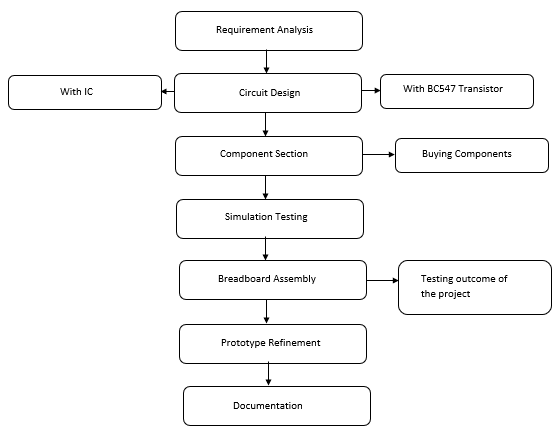
\includegraphics[width=0.5\textwidth]{workflow.png} % Replace 'diagram.png' with your image file
    \caption{Workflow}
    \label{fig:sample}
\end{figure}




\pagebreak
\subsection{Google Site}

\url{https://sites.google.com/diu.edu.bd/batterylevelindicator?usp=sharing}
\newline 
\newline
The circuit design is shown in Figure: 2.3.\newline
\begin{figure}[h!] % 'h' for placing it "here"
    \centering
    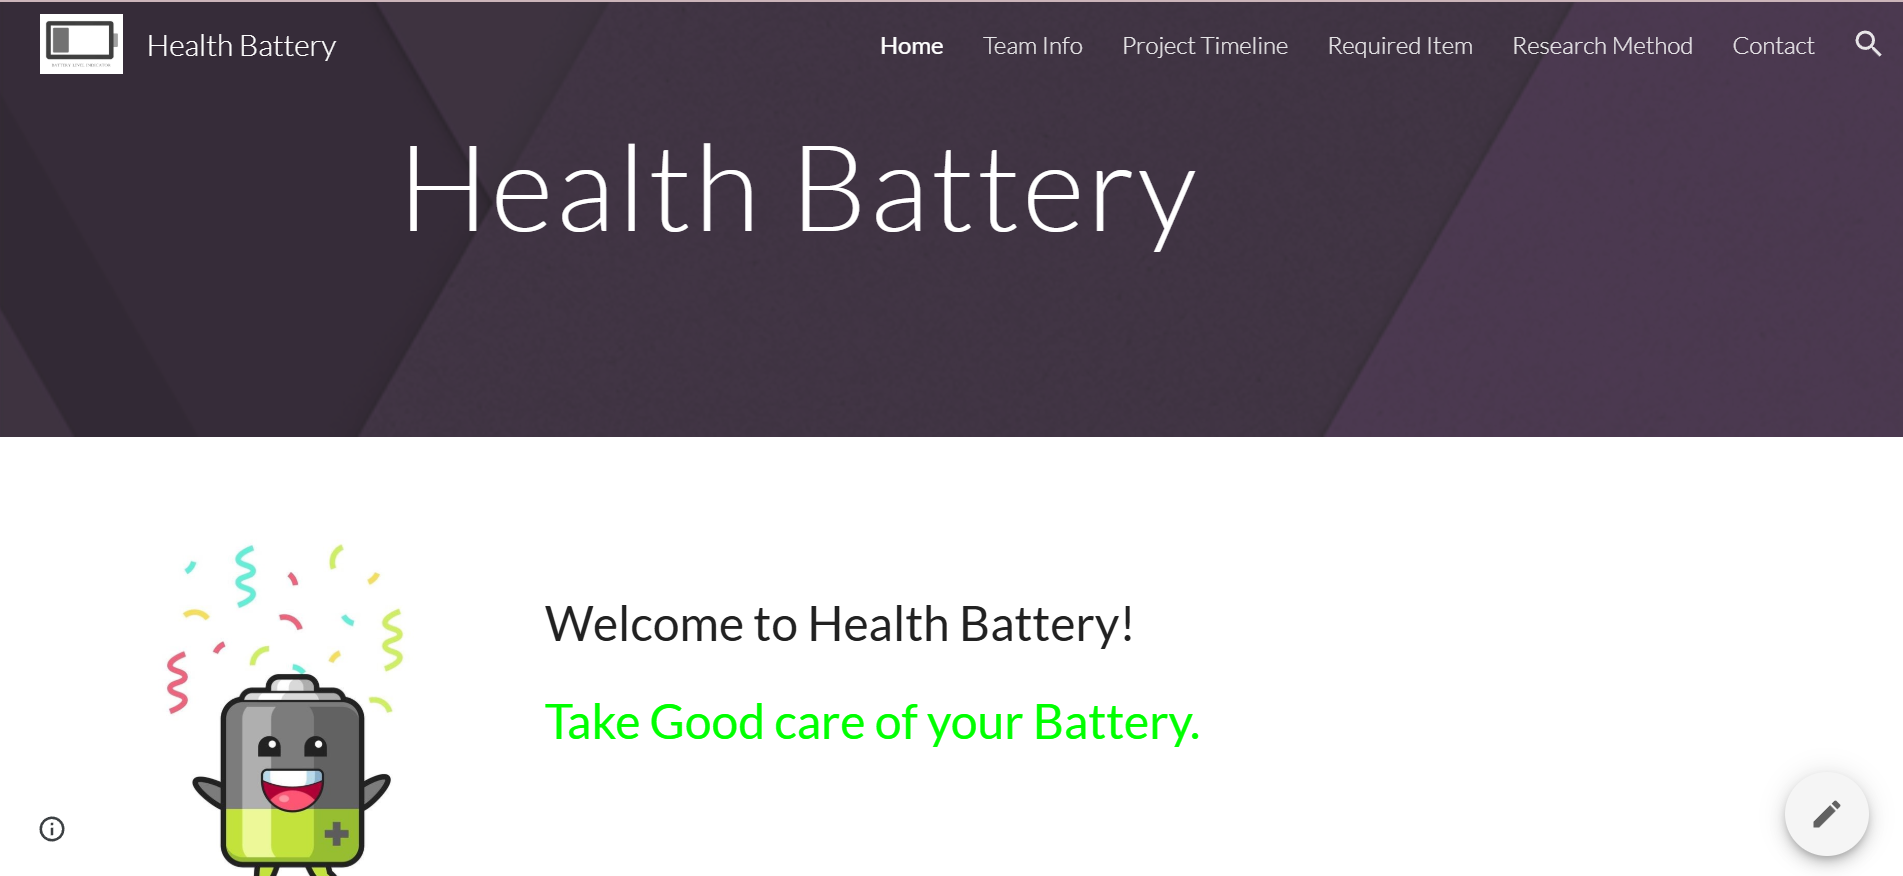
\includegraphics[width=0.5\textwidth]{1.png} % Replace 'diagram.png' with your image file
    \caption{Home Page of Google site}
    \label{fig:sample}
\end{figure}
\newline

The circuit design is shown in Figure: 2.4.\newline
\begin{figure}[h!] % 'h' for placing it "here"
    \centering
    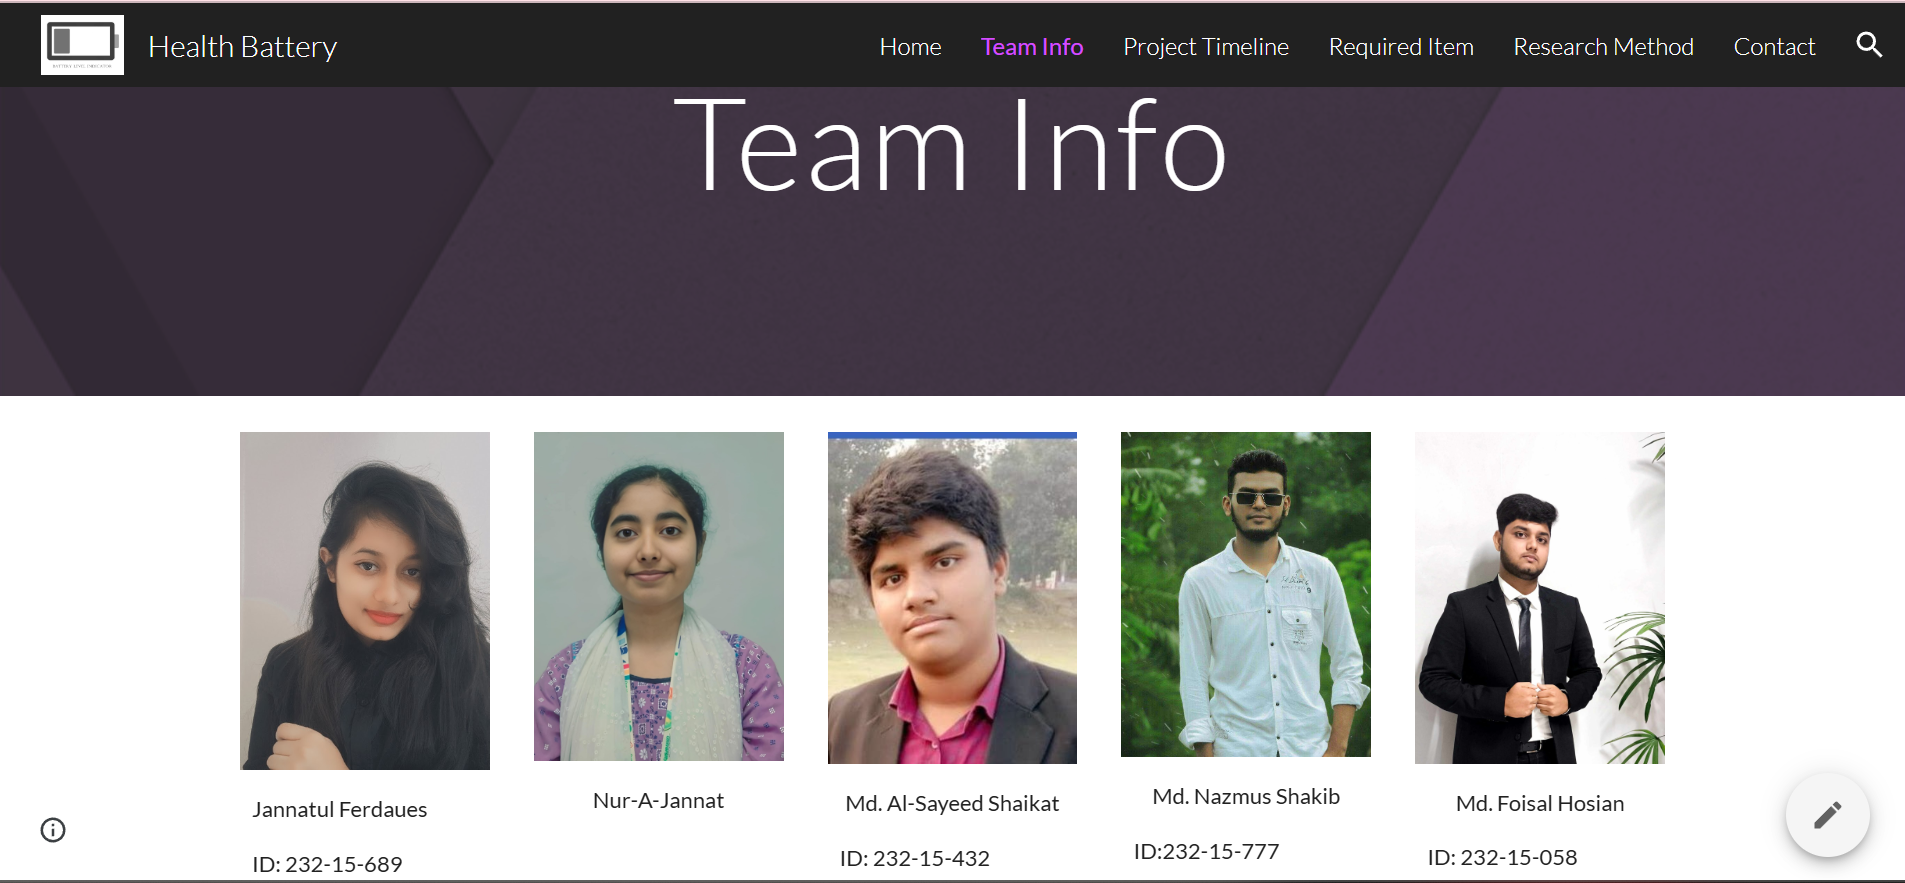
\includegraphics[width=0.5\textwidth]{2.png} % Replace 'diagram.png' with your image file
    \caption{team Info}
    \label{fig:sample}
\end{figure}

\newline The circuit design is shown in Figure: 2.5.
\begin{figure}[h!] % 'h' for placing it "here"
    \centering
    
\includegraphics[width=0.5\textwidth]{3.png} % Replace 'diagram.png' with your image file
    \caption{Time Duration}
    \label{fig:sample}
\end{figure}
\pagebreak
\newline The circuit design is shown in Figure: 2.6.
\begin{figure}[h!] % 'h' for placing it "here"
    \centering
    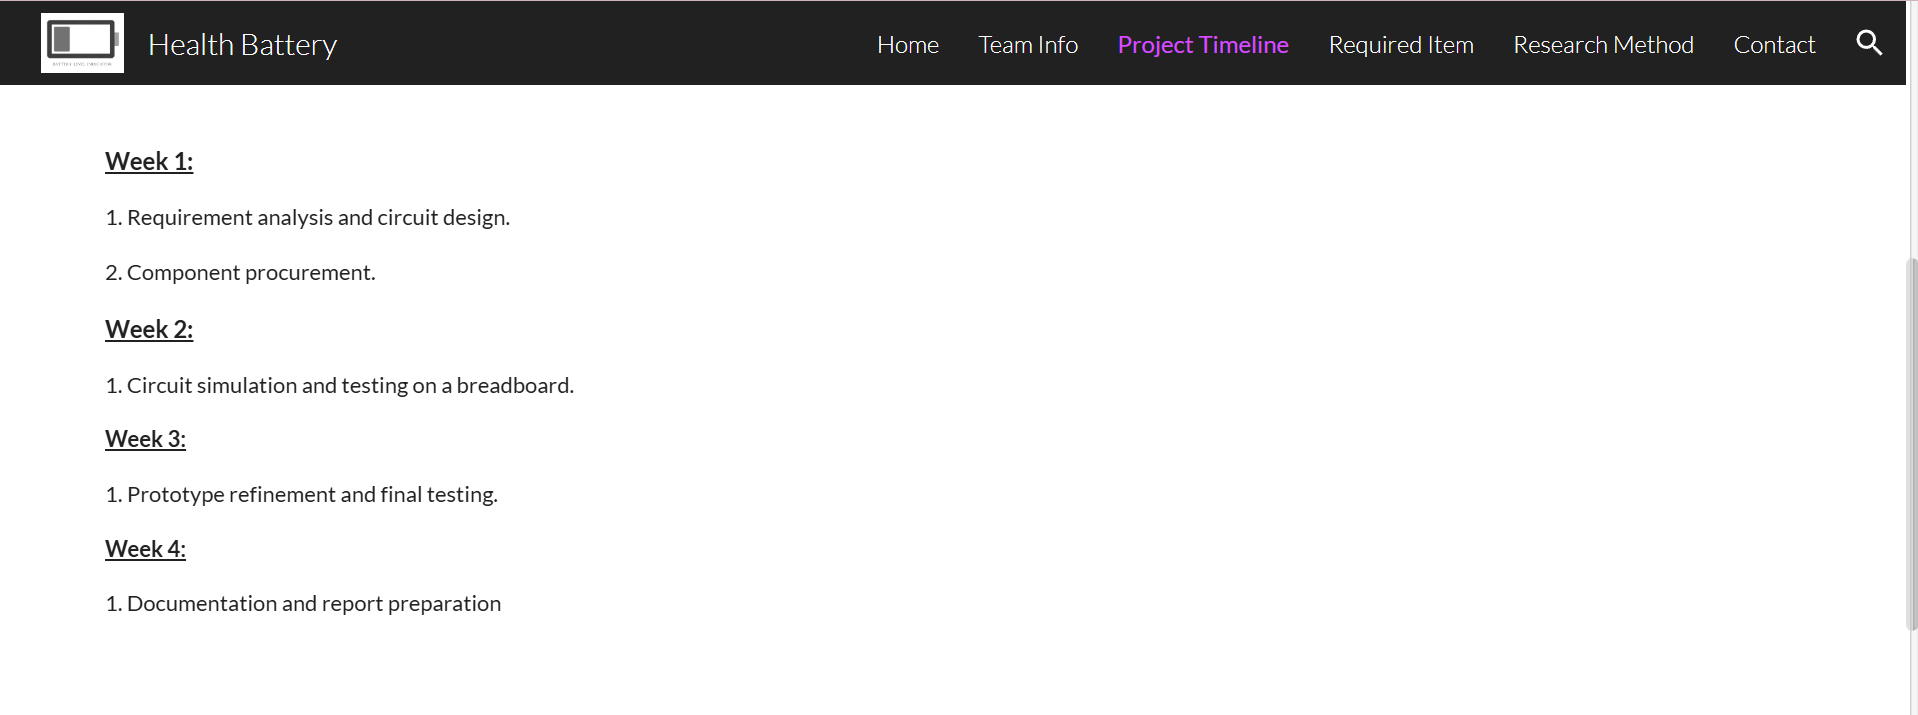
\includegraphics[width=0.5\textwidth]{4.png} % Replace 'diagram.png' with your image file
    \caption{Time Duration( weekly work)}
    \label{fig:sample}
\end{figure}

 \newline The circuit design is shown in Figure: 2.7.
\begin{figure}[h!] % 'h' for placing it "here"
    \centering
    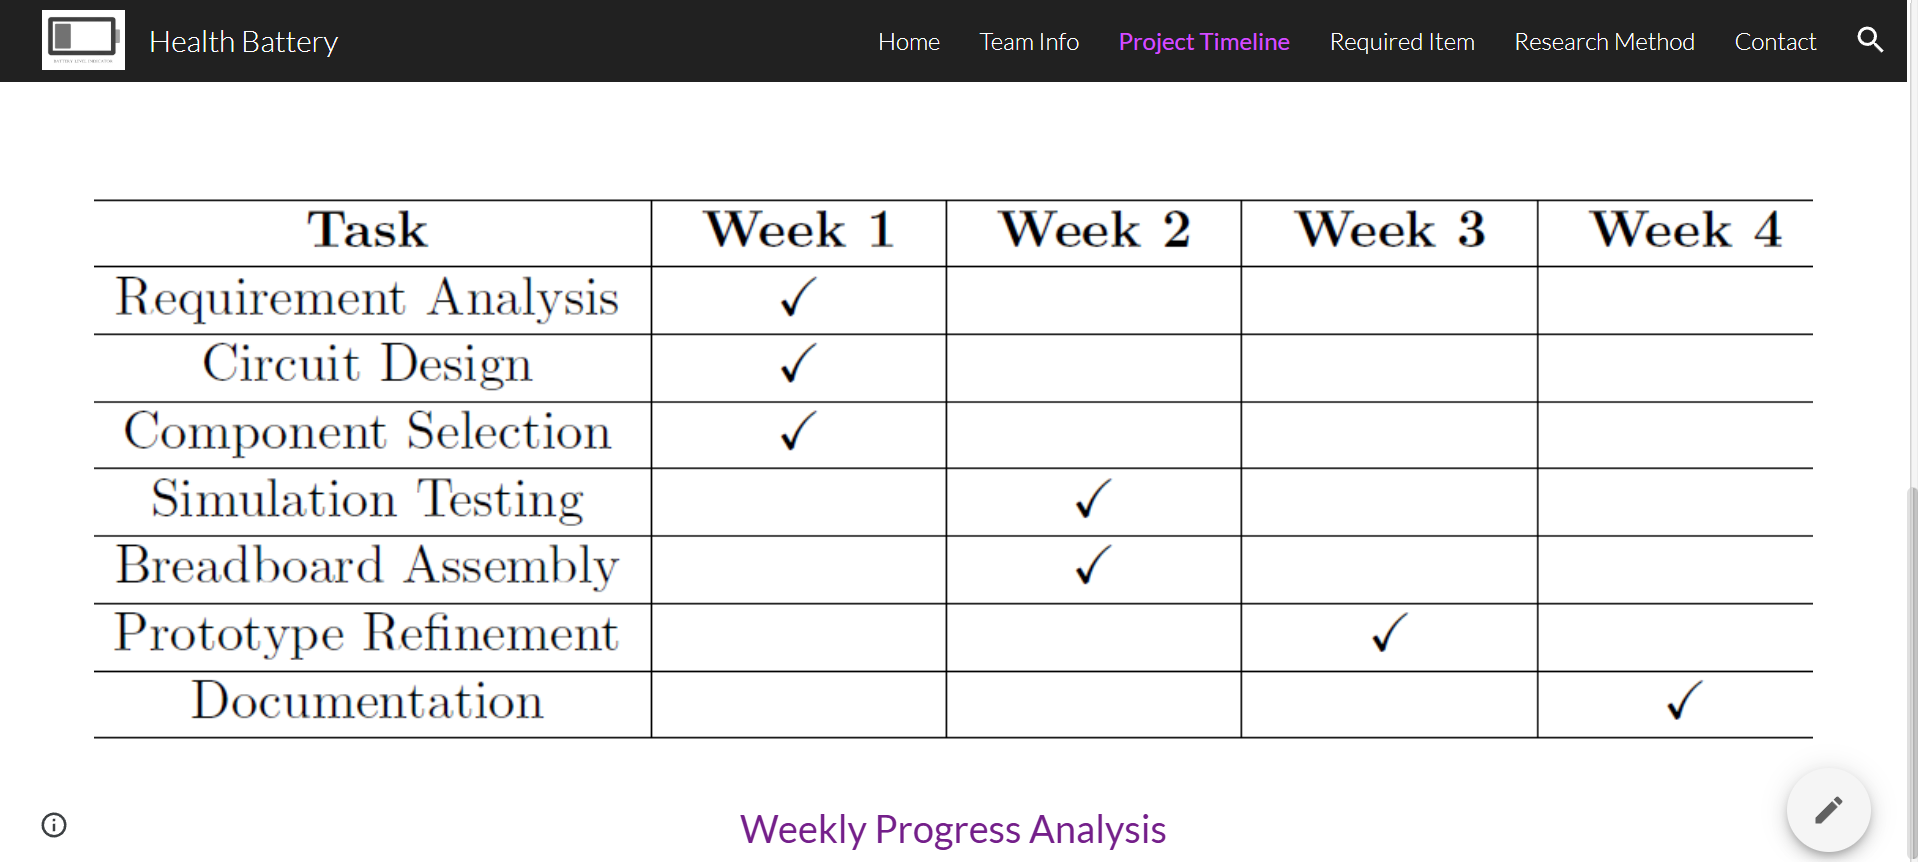
\includegraphics[width=0.5\textwidth]{5.png} % Replace 'diagram.png' with your image file
    \caption{Time Duration analysis}
    \label{fig:sample}
\end{figure}
 \newline The circuit design is shown in Figure: 2.8.
\begin{figure}[h!] % 'h' for placing it "here"
    \centering
    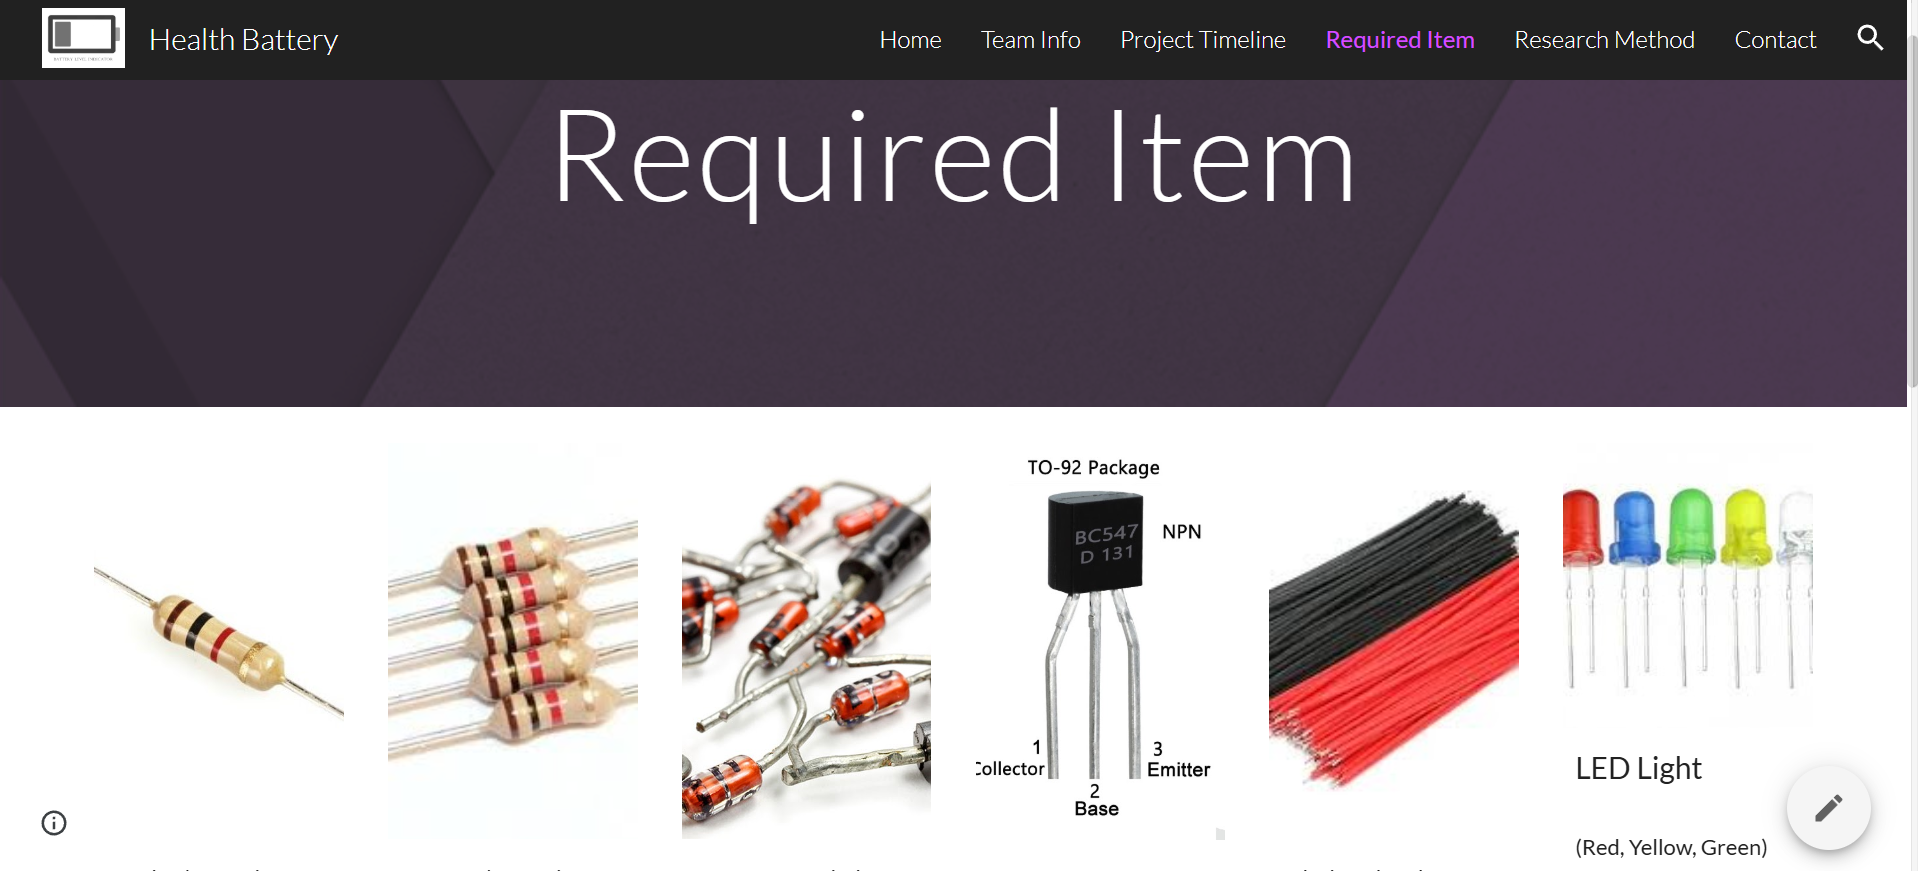
\includegraphics[width=0.5\textwidth]{6.png} % Replace 'diagram.png' with your image file
    \caption{Required Item}
    \label{fig:sample}
\end{figure}
\newline
 \newline The circuit design is shown in Figure: 2.9.
\begin{figure}[h!] % 'h' for placing it "here"
    \centering
    
\includegraphics[width=0.5\textwidth]{7.png} % Replace 'diagram.png' with your image file
    \caption{Research Method}
    \label{fig:sample}
\end{figure}
\newline
\pagebreak
 \newline The circuit design is shown in Figure: 2.10.
\begin{figure}[h!] % 'h' for placing it "here"
    \centering
    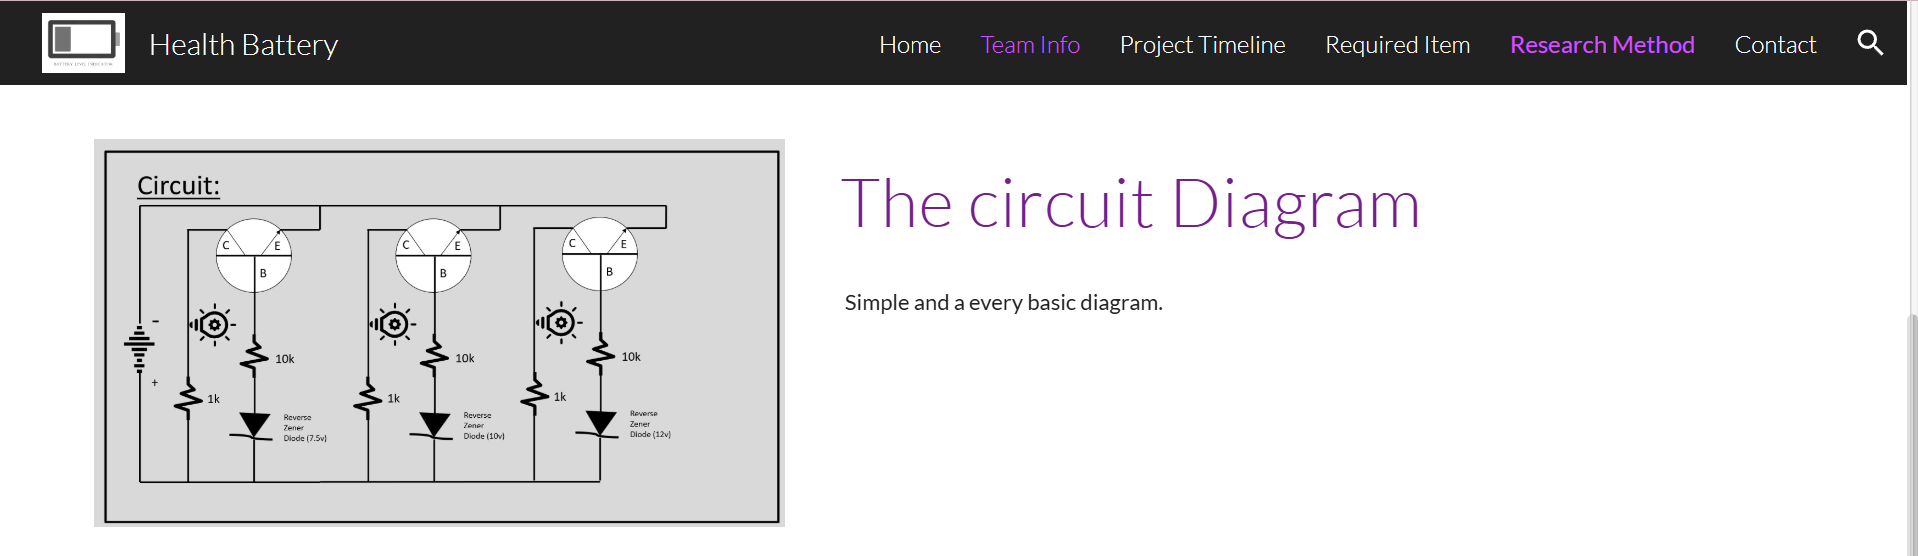
\includegraphics[width=0.5\textwidth]{8.png} % Replace 'diagram.png' with your image file
    \caption{Research Method (circuit diagram)}
    \label{fig:sample}
\end{figure}
 \newline The circuit design is shown in Figure: 2.11.
\begin{figure}[h!] % 'h' for placing it "here"
    \centering
    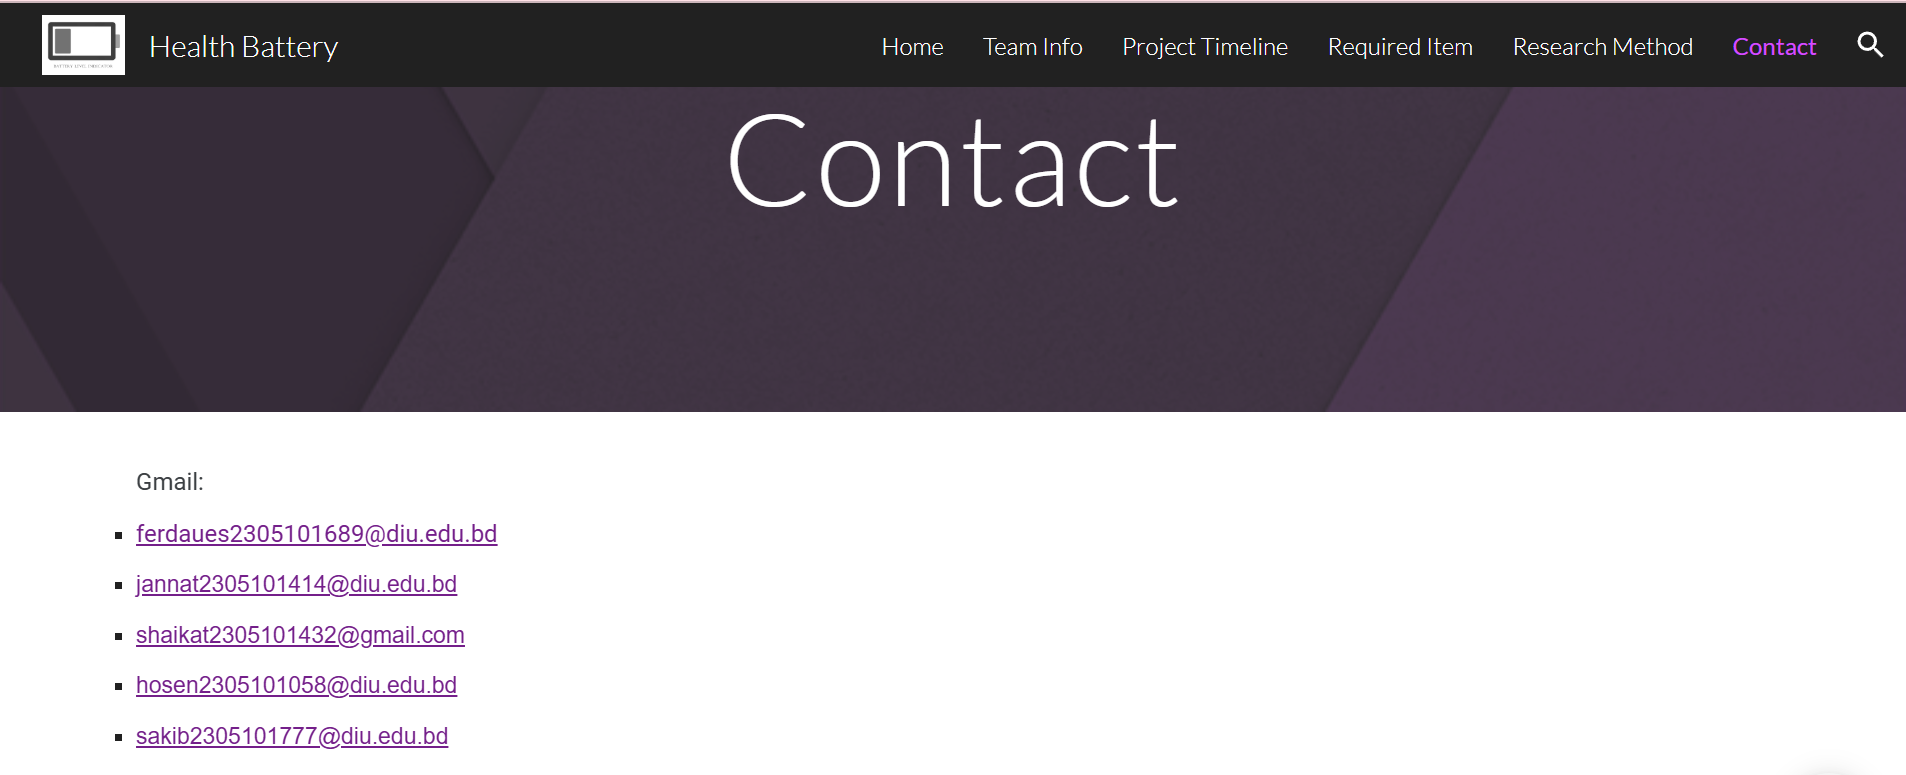
\includegraphics[width=0.5\textwidth]{9.png} % Replace 'diagram.png' with your image file
    \caption{Contact Info}
    \label{fig:sample}
\end{figure}


\section{Overall Project Plan}

The main reason is to create a simple and reasonable project. This can be designed using an IC . In modern-day electronics, rectifiers are used for the conversion of AC to DC voltage. The present investigation focuses on exploring the various rectifier circuits constructed using a transistor(BC547) instead of rectifier diodes (1N4007). Forward and reverse bias conditions of the diode were realized using transistors. Half-wave and full-wave rectifiers were constructed using transistors. The obtained output waveforms were compared with rectifier diode waveforms \cite{3}. 1k ohm resistors are used as current-limiting resistors for LEDs, and 10k ohm resistors are used as base resistors for the transistors. In this project, three different kinds of Zener diodes are used. The 7v Zener diode is used for low-volt detection, the 10v Zener diode is used for medium-range volt detection, and finally, the 12v Zener diode is used for high-voltage detection \cite{b1}.
\vspace{.1cm}

\begin{table}[h!]
\centering
\begin{tabular}{|  c  |c|c|c|c|}
\hline
\textbf{      Task      } & \textbf{  Week 1  } & \textbf{  Week 2  } & \textbf{  Week 3  } & \textbf{  Week 4  } \\
\hline
 Requirement Analysis &  \checkmark &   &   &  \\
\hline
 Circuit Design &  \checkmark &   &   &  \\
\hline
Component Selection & \checkmark &   &   &  \\
\hline
Simulation Testing &  & \checkmark  &   &  \\
\hline
Breadboard Assembly &  &  \checkmark &   & \\
\hline
Prototype Refinement &  &   &  \checkmark &  \\
\hline
Documentation &  &   &   & \checkmark \\
\hline
\end{tabular}
\caption{Weekly Progress Analysis}
\end{table}

\vspace{2cm}

\chapter{Implementation and Results}

In this chapter, you will be acquainted with the implementation of the electric circuit consisting of BC547 NPN transistors, LEDs, Zener diodes, and resistors. Also a  clear description of performance analysis and the outcomes of the experiment are also provided.
\end{center}

%This is for reference only. Delete before finalization

\section{Implementation}

This project is being done by building a circuit on a bread board. The objective is to illustrate how transistors can be used as switches to control LED states in response to the changing voltage applications. The components of the project include:
\newline \textbf{1. Three BC547 NPN transistors:}
\newline The path for the current through the LEDs is established by these transistors which act as switches. Current limiting the base of each transistor is done by the resistor attached to it and connections will be made from a separate LED to each of the transistors.\cite{b10}
\newline \textbf{2. Three LEDs (red, yellow, and green):} 
\newline Each of the LEDs represents a different circuit state. A red LED represents the lowest voltage, a yellow LED represents the moderate voltage, and the green LED heralds the greatest voltage.\cite{b12}
\newline \textbf{3. Resistors:}
\newline The base resistors for the transistors are three 10kΩ resistors that are connected in order to limit the current passing through the Governor to the transistor’s base.
\newline Three 1kΩ resistors are used as current-limiting resistors in order to prevent LEDs from being damaged by overload currents.
\newline \textbf{4.Zener Diodes:}
\newline The 7.5V Zener Diode is utilized to maintain the specified voltage which prevents the circuit from receiving voltage beyond the designated level.
\newline The 10V and 12V Zener Diodes are then used in order to have LEDs show their different response to different voltage levels. Zener diodes are used to produce a constant voltage that can supply the required voltage to the transistor circuits.
\newline 12V Battery: A 12V source is used in order to power the entire circuit. It is able to provide enough voltage for both the LEDs and the transistors.\cite{10}
\newline \textbf{5.Male to Male Jumper Wires:}
\newline These wires carry the current flow without soldering the breadboard components.
\newline In this way, transistors are arranged in a switching configuration, and the Zener diodes control the voltage supplied to each transistor's base. The LEDs are accordingly lightened as the voltage goes up/down at the base of the transistor which is in turn managed by the Zener diodes.




\section{Performance Analysis}

The circuit's performance is analyzed by measuring the current through the LEDs and the transistor's switching behavior under different conditions. Important performance outputs are:
\newline \textbf{LED Brightness:} The brightness of each LED is a method to check the transistor's performance as a switch and also shows the Zener diodes' voltage stability.\cite{b13}
\newline \textbf{Current Limiting:} The current through the LEDs and transistors is measured to see if it is within safe limits.\cite{9}
\newline \textbf{Voltage Regulation:} The Zener diodes are tried to confirm if they can control the volts at certain levels (7.5 V, 10 V, and 12 V) and, hence, protect the circuit.\cite{8}
\newline Different voltage environments are applied during tests to investigate the action of each part as well as their responsibility for regulating current and LEDs.

\section{Results and Discussion}

\textbf{The experimental results showed that:}
The zener diodes were very good in holding the voltage at the expected values (7.5 V, 10 V, and 12 V), thus the circuit was stable and protected.
The BC547 transistors, by working as effective switches, enabled the current to pass through LEDs when the correct voltage was applied to the base.
The LEDs thus are perfectly matched to changes in voltage, with the red LED shining at the lower voltages, and the green LED only comes on at higher voltages, thus, current control leads to effective voltage control.
1k resistors with current limiting characteristics worked just fine in avoiding overcurrent that would damage the LED lights and help to prevent the longevity of these semiconductors through burning out.
The experimental results attest to the design concepts that involve transistors and Zener diodes in the LED-based system. Additionally, the design offers the possibility of optimization of different voltage levels and the use of additional LEDs or components.\cite{b16} Some pictures of the project in working state is given below-
\newline
The Red LED is glowing when 7.5 volt current is passing.It is shown in Figure: 3.1.
\begin{figure}[h!] % 'h' for placing it "here"
    \centering
    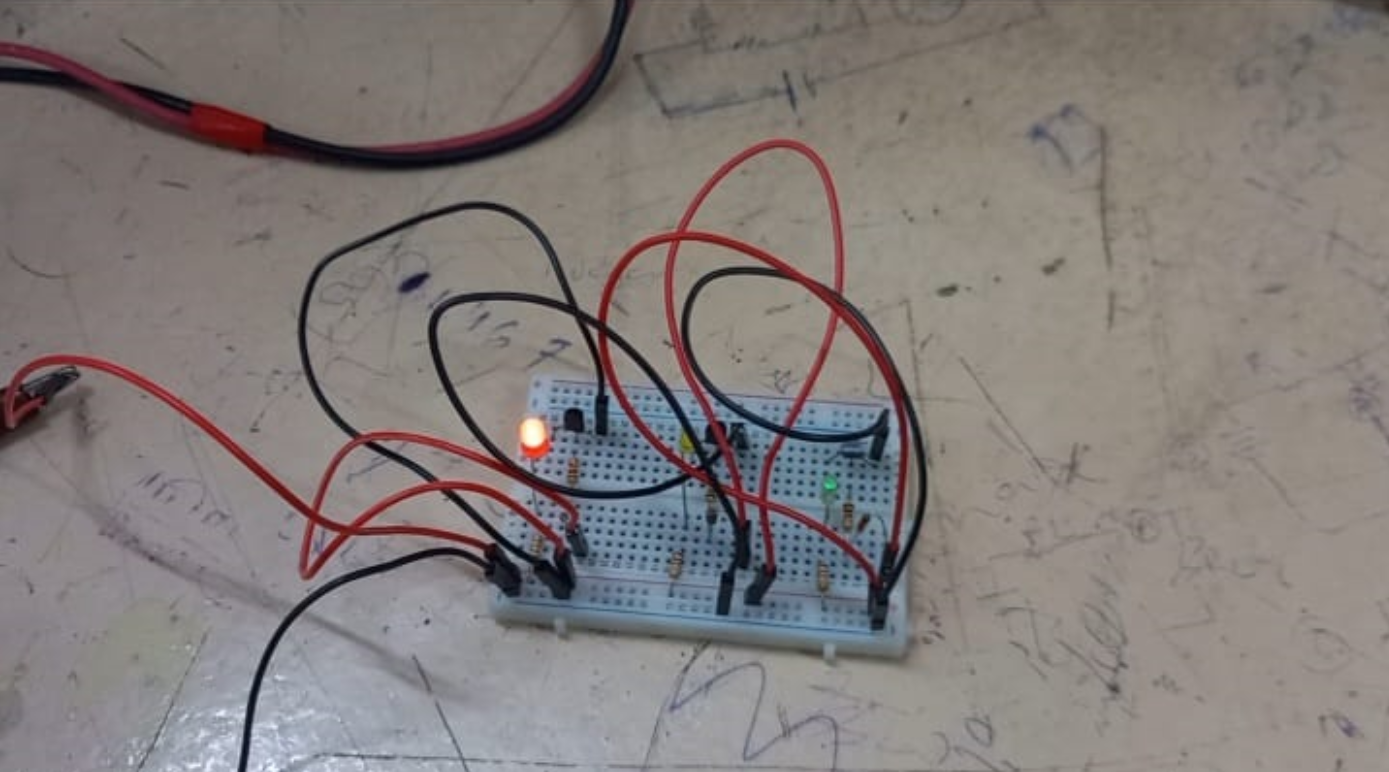
\includegraphics[width=0.5\textwidth]{10.png} % Replace 'diagram.png' with your image file
    \caption{Research Method}
    \label{fig:sample}
\end{figure}

\pagebreak
 The red and yellow LEDs are glowing when 10 volt is given.It is shown in Figure: 3.2.
\begin{figure}[h!] % 'h' for placing it "here"
    \centering
    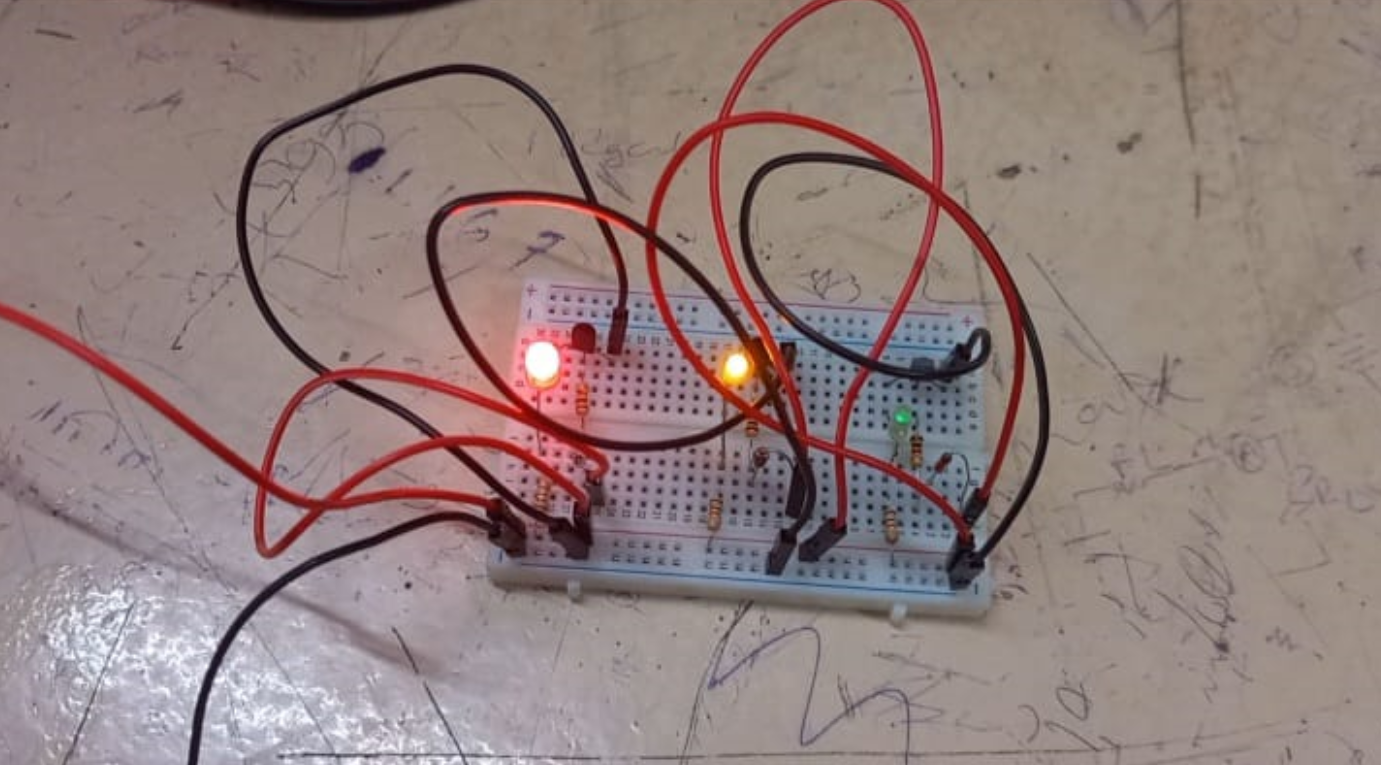
\includegraphics[width=0.5\textwidth]{11.png} % Replace 'diagram.png' with your image file
    \caption{Research Method}
    \label{fig:sample}
\end{figure}
\newline
All LEDs are glowing when 12 0r more volt is given.It is shown in Figure: 3.3.
\begin{figure}[h!] % 'h' for placing it "here"
    \centering
    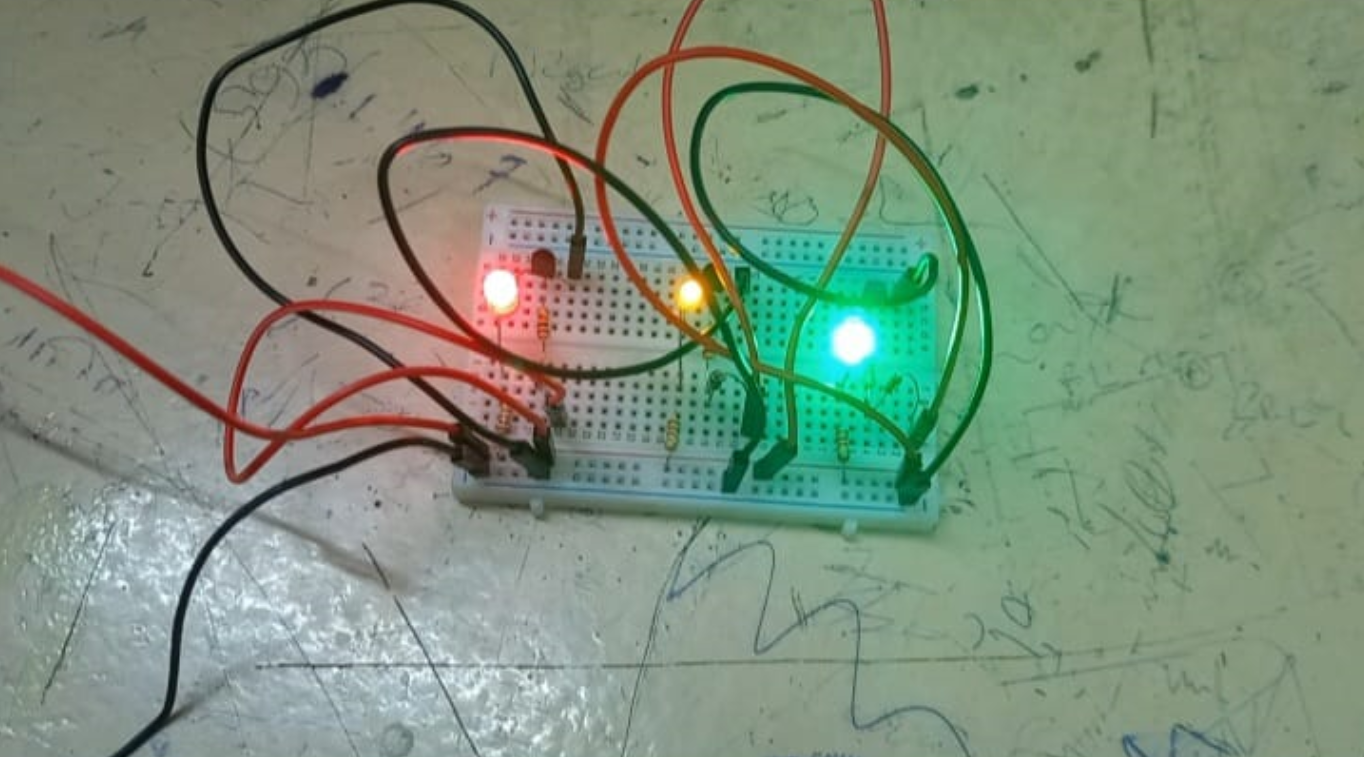
\includegraphics[width=0.5\textwidth]{12.png} % Replace 'diagram.png' with your image file
    \caption{Research Method}
    \label{fig:sample}
\end{figure}

\chapter{Engineering Standards and Mapping}


This chapter presents the engineering standards and practices that were used to develop and implement the electronic circuit. It covers the larger/social effects of the project such as its sustainability and ethical issues that it may create. Apart from that, the chapter includes the project management issues such as cost analysis, revenue models and teamwork by mapping the engineering problem to program outcomes.
\end{center}
%This is for reference only. Delete before finalization

\section{Impact on Society, Environment and Sustainability}

In this chapter, you will be acquainted with the implementation of the electric circuit having BC547 NPN transistors, LEDs, Zener diodes, and resistors. A clear description of performance analysis and the outcomes of the experiment are also provided.

\subsection{Impact on Life}

The circuit that is built using transistors, resistors, LEDs, and Zener diodes, besides proving a model for the demonstration of electronic components, shows how well these devices work in practice, thus, it also supports the understanding of the basic principles of electrical engineering. That kind of a project can develop knowledge especially in the educational programs where student’s practical learning of transistor switching circuits improves the understanding of electronics. They are real projects that bring on designs and applications that are more eco-friendly by applying low-cost, energy-efficient circuits.

\subsection{Impact on Society \& Environment}


Per a ‘strictly’ social point of view, the use of this technology provides a remarkable, capabilities-of-electronic-circuits-in-home-automation-and-industrial-applications, including voltage, applications of popular motors and the application of electronic circuits for performing industrial tasks and business production. Its power-saving and the fact that it is easy enough to be carved from stone, make it possible to be discarded without a footprint and hence, forever vanish from nature, it is therefore a projectile or a shuttle for teaching and experiment work.
The circuit in the environmental setting is based on a 12V battery source to ensure that the elements eat less, thereby reducing the waste. Also, charts which provide a generative model for design highly reducing production, can be modified or customized according to different needs, thus e-Waste control can be effectuated.\cite{b17}

\subsection{Ethical Aspects}

In terms of ethics, the determination of resistors and Zener diodes by the right choice, thereby limiting the overcurrent and voltage spikes which might otherwise damage the circuit is indeed the safety that has been ensured. The project also takes into account the safe battery handling and disposal aspect which would curb the environmental pollution. In addition to that, the low-power components and materials that are reusable for the breadboard, materials that are used in a way of ethical way, are also an important part of the logic behind the design or assemblage.

\subsection{Sustainability Plan}

To improve the project's sustainability, the used components (resistors, transistors, diodes) are easily, cheaply, and widely available which in turn, decreases the environmental cost of production and distribution. Besides, the design by using the materials that are slaughtered en masse like breadboards and jumper wires, the design is convenient and easy to alter and convert for later projects thus even longer life and wider utilization is ensured. To add to that, the design by using the materials that are handy and cheap such as breadboards and jumper wires which are easy to procure and certainly green, is fine for jobs that require only replacement through easy modifications and redesigns of future projects.\cite{b18}


%\section

\section{Project Management and Team Work}


This entire project was based on effective project management and teamwork. Each member was involved in the initial brainstorming sessions to the final test of the circuit; he or she contributed his or her expertise and knowledge so well to deliver the project requirements efficiently and on time. There were ongoing regular communications, delegations of tasks, and problem-solving that were worth the cost of overcoming challenges in the timely-progress toward completion. This collaborative approach was the key to a successful balancing of cost, functionality, and performance within this project.
\vspace{.5 cm}
\newline\textbf{Teamwork Dynamics:}
It was a big task that was well planned with every member of the team taking responsibility for research and sourcing of components that could be made cheaper but of quality, with many checks on the price not sacrificing the performance of the circuit. The team determined once more the necessary components and avenues to cut costs for the circuit to fulfill its functional goals. The analysis also reveals the itemized costs reflecting individual and team decisions:
\newline\textbf{1.Breadboard:} - It was selected due to its ease of use and reuse; it proved critical in prototyping the circuit.
\newline\textbf{2.BC547 NPN Transistors (3 pcs):} - The transistors were chosen because they are very cheap and quite good at switching LEDs on and off.
\newline\textbf{3.LEDs (Red, Yellow, Green):} - A set of three LEDs can glow depending on the voltage.
\newline\textbf{4.Resistors (1kΩ, 10kΩ):} The right resistors were chosen with group members working together to make sure the appropriate current flow and voltage regulation.
\newline\textbf{5.Zener Diodes (7.5V, 10V, 12V):} - The zener diodes were selected to regulate the voltage at certain levels so that the transistors operate within their safe operating limit.
\vspace{.5 cm}
\newline The cost breakdown indeed shows how a collective decision from the team assisted the team in strategic component selection and saving in cost without affecting circuit performance. As a team group, they assessed alternatives like making use of fewer components or a cheaper power supply, but finally came to the conclusion that the components they had chosen were the most ideal ones considering their performance to price ratio.\cite{b19} A table is given below showing each members contribution on making this paper-

\begin{table}[h!]
\centering
\caption{Course Outcome Statements}
\vspace{0.1cm} % Adds a 0.5 cm space between the caption and the table
\begin{tabular}{|p{0.02\textwidth}|p{0.3\textwidth}|p{.6\textwidth}|}
\hline
\textbf{SI} & \textbf{Team Member Name} & \textbf{Contributions} \\
\hline
1 & Nur-A-Jannat & Chapter-1(Introduction) \\
\hline
2 & Jannatul Ferdaues & Chapter-2(Proposed Methodology/Architecture) \\
\hline
3 & MD Faisal Hosen & Chapter-3(Implementations and Results)\\
\hline
4 & MD AL Sayeed Shaikat & Chapter-4(Engineering Standards and Mapping)\\
\hline
5 & MD Nazmus Sakib & Chapter-5(Conclusion)\\
\hline
\end{tabular}
\end{table}

\noindent\textbf{Alternative Budgeting and Team Decision Making:}
The team would have reduced the number of transistors had it been more tight on the budget or could have resulted in a cheaper power source. However, the team felt they should stick with the same design for a better educational value since the concept of multiple transistor use and voltage regulation needed to be used as part of the learning experience. It is this kind of decision-making scenario that reflects teamwork dynamics, as each team member brought in their views about making optimum designs in functionalities and possible costs. The actual expenses reflect the contribution by the group to ensure that the project becomes affordable for educational purposes while keeping the technical requirements.
\vspace{.5 cm}
\newline\textbf{Revenue Model and Collaborative Strategy:}
In the case of a scaled project for commercial or educational application, the team considered some future streams for revenue generation, using which their collaborative effort would be useful in pinpointing target markets, developing materials for instruction, and constructing pricing strategies. Key items of the revenue model would include:
\vspace{.5 cm}








 

\section{Complex Engineering Problem}

This section addresses the complexity of the engineering challenge tackled by the project. It includes the process of integrating various components into a working circuit and how engineering standards were applied.

\subsection{Mapping of Program Outcome} 

The project aligns with the following Program Outcomes (POs) that assess the skills developed during the project:

\begin{center}
    \begin{table}[ht]
        \centering
        \caption{Justification of Program Outcomes}
        \begin{tabular}{|p{0.2\textwidth}|p{0.7\textwidth}|}
            \hline
            \textbf{PO's} & \textbf{Justification} \\
            \hline
            PO1 & Engineering Knowledge.  \\
            \hline
            PO2 & Problem Analysis. \\
            \hline
            PO3 & Design/Development of Solutions. \\
            \hline
        \end{tabular}
        \label{tab:po_justification}
    \end{table}
\end{center}



\subsection{Complex Problem Solving} 

The engineering challenge involved solving multiple conflicting requirements, such as selecting the correct resistors to ensure both voltage regulation and current control while keeping the circuit simple and cost-effective. The mapping table below illustrates the complexity of the problem-solving process:\cite{b20}. The table for complex problem-solving is shown in Table 4.2. 

    \begin{table}[ht]
        \centering
        \caption{Mapping with complex problem-solving.}
        \begin{tabular}{|p{0.12\textwidth}|p{0.12\textwidth}|p{0.12\textwidth}|p{0.12\textwidth}|p{0.12\textwidth}|p{0.12\textwidth}|p{0.12\textwidth}|}
        \hline
        EP1& EP2& EP3& EP4& EP5& EP6& EP7\\
        Dept of Knowledge & Range of Conflicting Requirements & Depth of Analysis & Familiarity of Issues & Extent of Applicable Codes & Extent of Stakeholder Involvement & Inter-dependence\\
        \hline 
        This problem requires knowledge in basic electronics, including the understanding of transistors, LEDs, resistors, and diodes, and how to integrate these components into a functional circuit.\newline $\sqrt{}$ & Balancing cost, power efficiency, and accurate voltage detection while ensuring user safety and ease of use.\newline $\sqrt{}$ & Moderate analysis is required to select appropriate Zener diodes and resistor values to ensure proper voltage division and LED signaling.\newline $\sqrt{}$ & The issues encountered are common in electronic circuit design, with familiarity in basic component functions and troubleshooting methods.\newline $\sqrt{}$
        &&&\\
        &&&&&&\\
        \hline 
        \end{tabular}
        \label{tab:p_solve}
    \end{table}


\pagebreak
\subsection{Engineering Activities}
 It actually includes field activities like iteration with theory in practical solving problems regarding electronics. Some specific activities include selection of components, circuit design, and validation of functional requirements.\cite{7}The table for complex engineering activities is shown in table 4.3.
\begin{center}
    \begin{table}[ht]
        \centering
                \caption{Mapping with complex engineering activities.}
        \begin{tabular}{|p{0.18\textwidth}|p{0.18\textwidth}|p{0.18\textwidth}|p{0.18\textwidth}|p{0.18\textwidth}|}
        \hline
        EA1& EA2& EA3& EA4& EA5\\
        Range of resources & Level of Interaction & Innovation & Consequences for society and environment & Familiarity\\
        \hline 
        The project uses readily available and low-cost resources such as BC547 transistors, resistors, and LEDs, making it an accessible project for many users.\newline $\sqrt{}$ & Interaction between components, including transistors, LEDs, and Zener diodes, requires careful consideration of the power supply and signal handling.\newline $\sqrt{}$ & The innovative aspect lies in the integration of simple components to create an efficient, reliable, and user-friendly battery monitoring solution.\newline $\sqrt{}$ & The project has positive implications for efficient battery management and sustainability by promoting proper charging and usage habits.\newline $\sqrt{}$ &\\
        &&&&\\
        \hline 
        \end{tabular}
        \label{tab:e_act}
    \end{table}
\end{center}

\chapter{Conclusion}

%This is for reference only. Delete before finalization
\begin{flushleft}

This chapter summarizes the entire project, its limitations, and future directions. Reflections are made around the achievements of this project, obstacles that were faced during the implementation, and any feasible further development opportunities.
\end{center}
%This is for reference only. Delete before finalization

\section{Summary}
The project involves designing and building a very basic electronic circuit using breadboard, BC547 NPN transistors and LEDs, few resistors, Zener diodes and a 12V battery. The concept behind it is to have a very simple voltage regulated switching arrangement, to show that an electronic switch by using transistors can be switched on and off with a voltage applied between two different levels. LEDs do indicate these switching operations. The objective of this project was achieved and all components are working together to realize a simple but functional circuited concept of voltage regulation, current limiting and switching by transistor.
Through practical learning experience by itself, the project outcome practically enlightens one not only physically towards electronics but would imply how simple components could also link towards developing a formed circuit using fundamental components into different applications, like home automation kits and education-based kits.\cite{b23}

\section{Limitation}

The project has many setbacks that cannot be concealed with the achievements and must be stated clearly:
\newline\textbf{1.Component Limitations:} Use of standard components like the BC547 transistor and Zener diodes rated for the power input into a circuit places a limitation when working under higher voltage or currents, thus future iterations may involve the use of power components for applications or systems much more complex and with higher power requirements.
\newline\textbf{2.Extent and Working:} This project used quite a simple circuit with few components making it very good for educational purposes only; however, for commercial use or scaling it up into high-end applications, power management, heat dissipation, and advanced voltage regulation options need to be considered very carefully.
\newline\textbf{3.Energy Efficiency:} This is energy efficient for educational purposes but it can actually not be a great improvement in the long run because of the 12V battery; long term or huge installations will therefore need either improved energy efficiency when it comes to the source or improved optimization of the circuit.
\newline\textbf{4.Limited Testing:} The testing environment was limited in terms of resources and simplicity of design. The scope of the project did not include more complex scenarios of testing with different kinds of loads or other types of voltage conditions.\cite{6}

\section{Future Work}

There is still a lot of innovation and extension that can be made to this project.
\newline\textbf{1.Improvement in Power Sources :} This becomes the project with renewable energy use, as it will use rechargeable batteries or solar panels as the energy source which will be used outdoors or off-grid. 
\newline\textbf{2.Expansion of Circuit Components:} Further development can be done with advanced components such as integrating microcontrollers or sensors to allow for the system's automation or remote control because this provides a closer approach to actual applications such as home automation systems.
\newline\textbf{3.Commercialisation and Personalisation:} This would probably constitute a leap into commercialisation for the project since it would possess scalability due to kit of component customization features such as variable voltage levels to multiple channels, thus appealing to a much wider market of hobbyists and educationists. 
\newline\textbf{4.Energy Management systems:} By using some modern energy management techniques like the improved voltage regulators or current buffers, the system would then be able to adopt larger loads or become more efficient in power consumption. So, it can widen the range of application for the circuit. 
\newline\textbf{5.Educational Extension:} It also might serve as an improvement for the curriculum in which the students might modify or enhance the circuit designs as per certain requirements so that they learn more and innovate into basic electronics.\cite{5,b26}




% References section
\renewcommand\bibname{References} % Ensure "References" title
\addcontentsline{toc}{chapter}{References} % Add "References" to TOC
\bibliographystyle{unsrt}
\bibliography{fydp} % Make sure fydp.bib exists in the same directory

\clearpage

\end{document}
